\documentclass[tikz]{standalone}
\usepackage[utf8]{inputenc}
\usetikzlibrary{calc,intersections}

\definecolor{DarkBlue}{rgb}{0.0,0.0,0.6}

\begin{document}

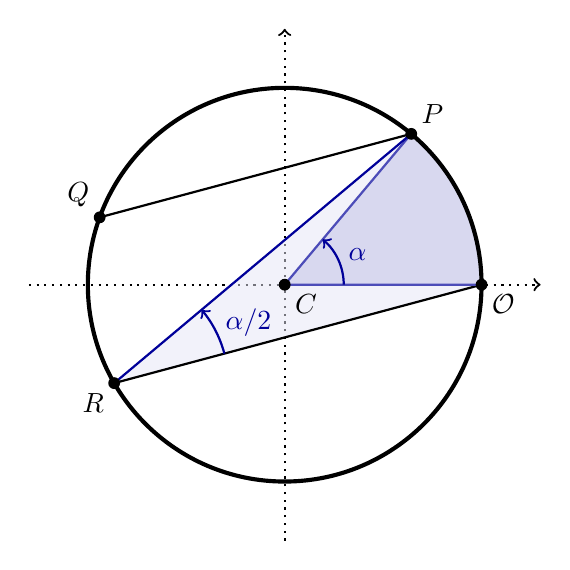
\begin{tikzpicture}[thick,scale=2.5]
\def\ptsize{.03}
\newcount\Pangle
\newcount\Qangle
\newcount\Rangle
\Pangle=50
\Qangle=160
\Rangle=\Pangle
\advance\Rangle by \Qangle
\draw[->,dotted] (-1.3, 0) -- (1.3,0);
\draw[->,dotted] (0,-1.3) -- (0,1.3);

\coordinate[label=below right:$\mathcal{O}$] (inf) at (1,0);
\coordinate[label=above right:$P$] (P) at (\number\Pangle:1);
\coordinate[label=above left:$Q$] (Q) at (\number\Qangle:1);
\coordinate[label=below left:$R$] (R) at (\number\Rangle:1);
\coordinate (C) at (0,0);

\fill[DarkBlue!10,opacity=.5] (R) -- (inf) -- (C) -- (P) -- cycle;
\fill[DarkBlue!30,opacity=.5] (C) -- (inf) arc (0:\number\Pangle:1) -- cycle;

\path[draw,name path=circ,line width=1.5pt] (0,0) circle (1);

\draw (P) -- (Q);
\draw (inf) -- (R);

\draw[line width=.8pt,DarkBlue!70] (P) -- (C) -- (inf);
\draw[line width=.8pt,DarkBlue] (P) -- (R);
\draw[DarkBlue,line width=.8pt,->] (.3,0) arc (0:\number\Pangle:.3) node[midway,right,yshift=2pt] {$\alpha$};
\draw[DarkBlue,line width=.8pt,->] ($(R)!.3!(inf)$) arc (15:40:.58) node[midway,right,yshift=3pt] {$\alpha/2$};

\fill (inf) circle (\ptsize);
\fill (P) circle (\ptsize);
\fill (Q) circle (\ptsize);
\fill (R) circle (\ptsize);
\fill (C) circle (\ptsize);
\node[below right] at (C) {$C$};
\end{tikzpicture}

\end{document}